\chapter{Tabele cu rezultate}

\begin{figure}
    \centering
    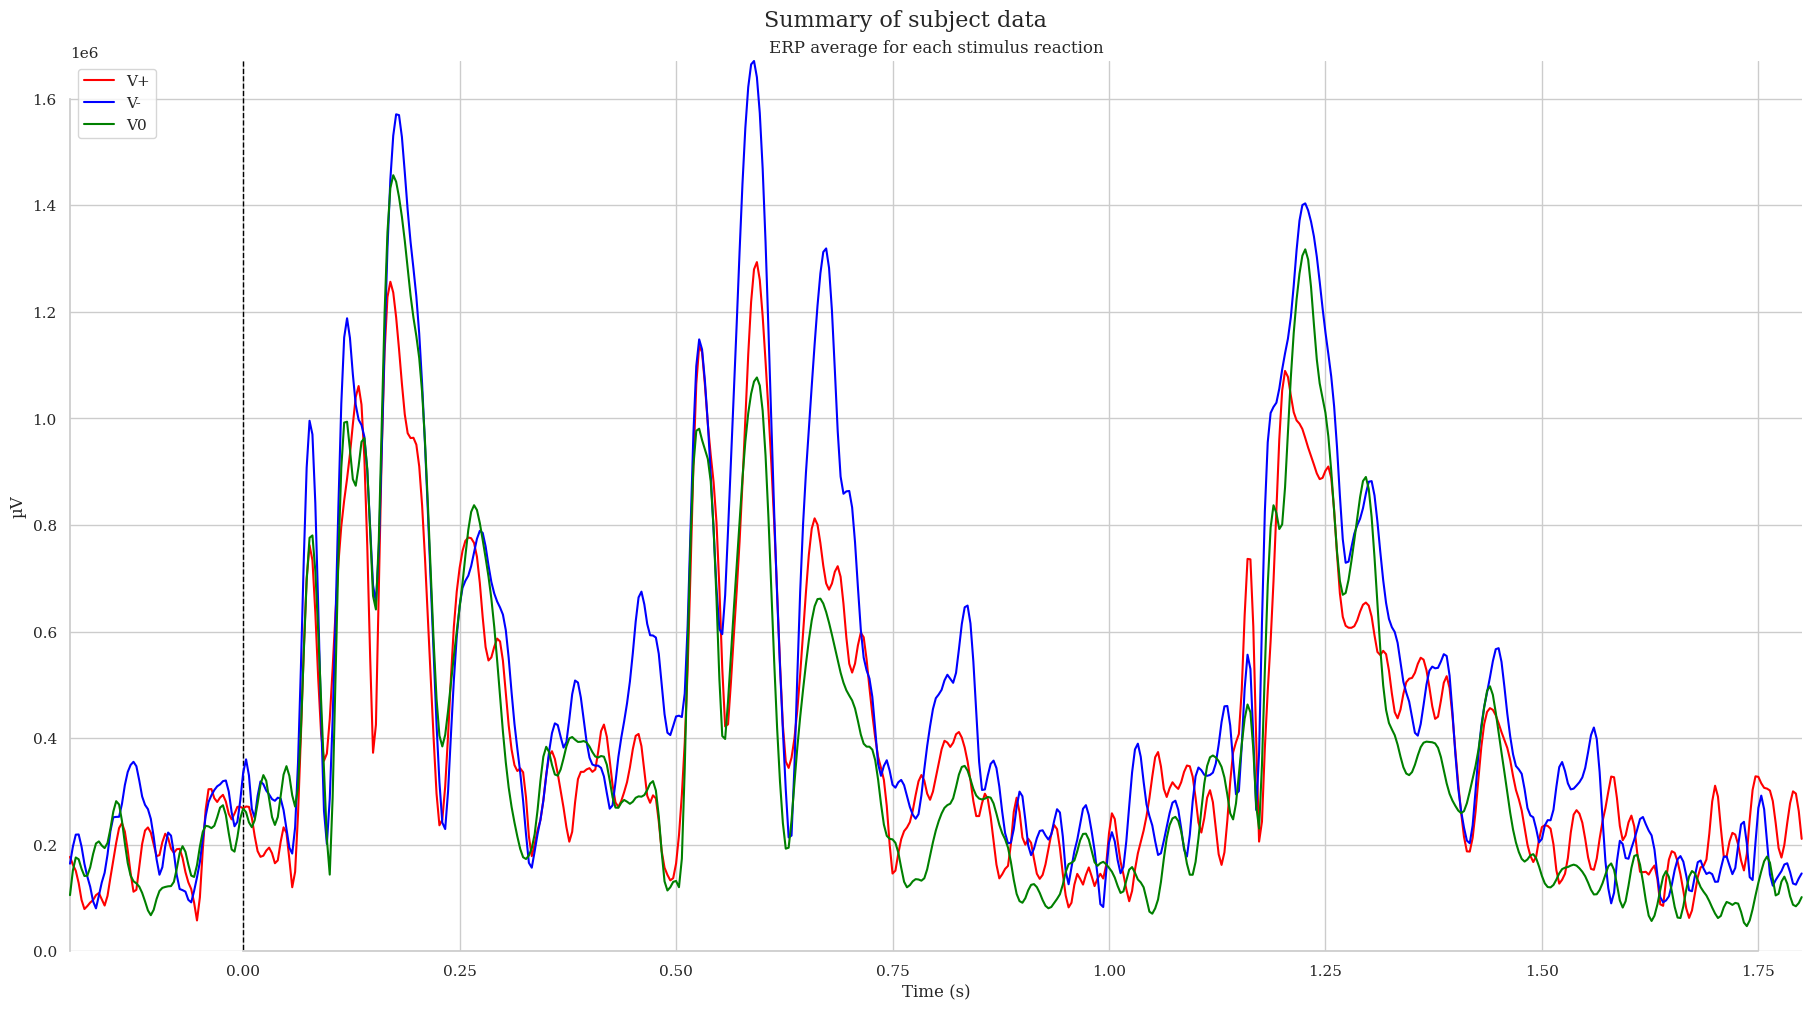
\includegraphics[width=1\linewidth]{images/average_response_each_erp.png}
    \caption{Raspunsul mediu pentru fiecare tip de eveniment.}
    \label{fig:average_response_by_event}
\end{figure}

\begin{figure}[h]
    \centering
    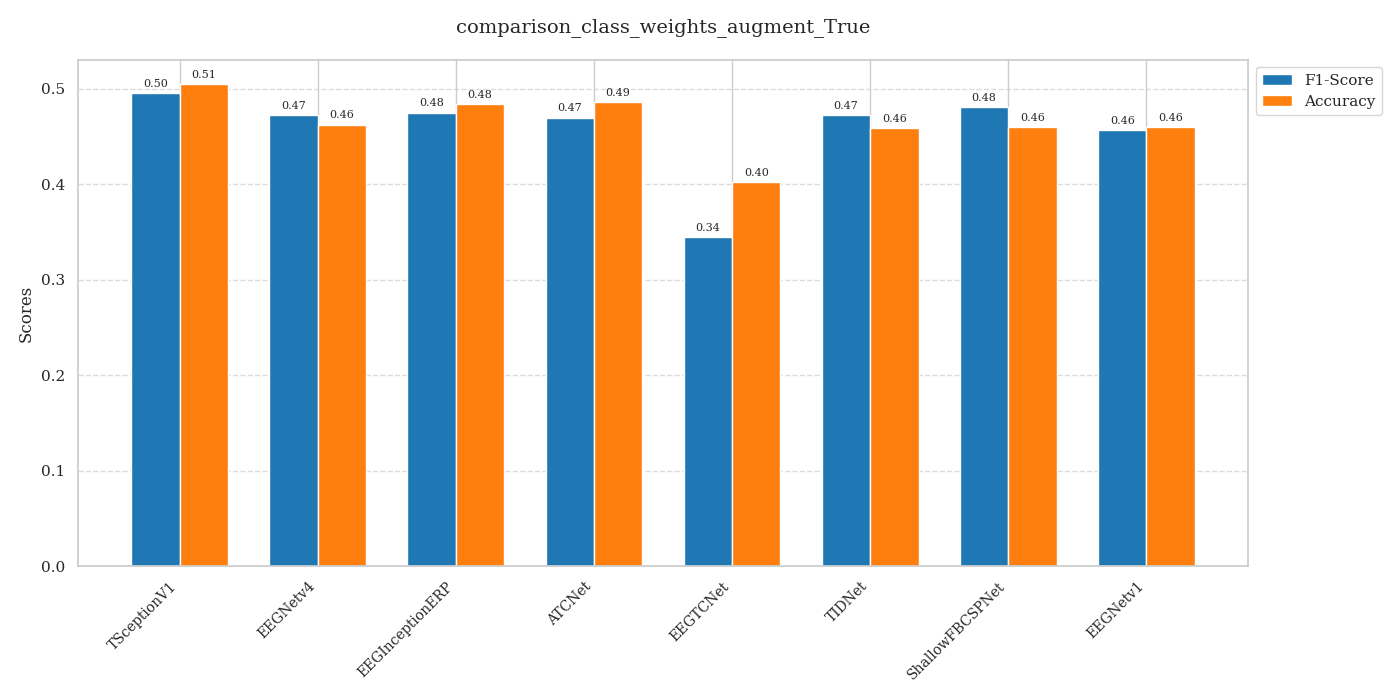
\includegraphics[width=1\linewidth]{images/comparison_class_weights_augment_True.png}
    \caption{Performanta modelelor cu weight-uri de clase si augmentari.}
    \label{fig:performance_class_weights_augment_true}
\end{figure}

\begin{figure}
    \centering
    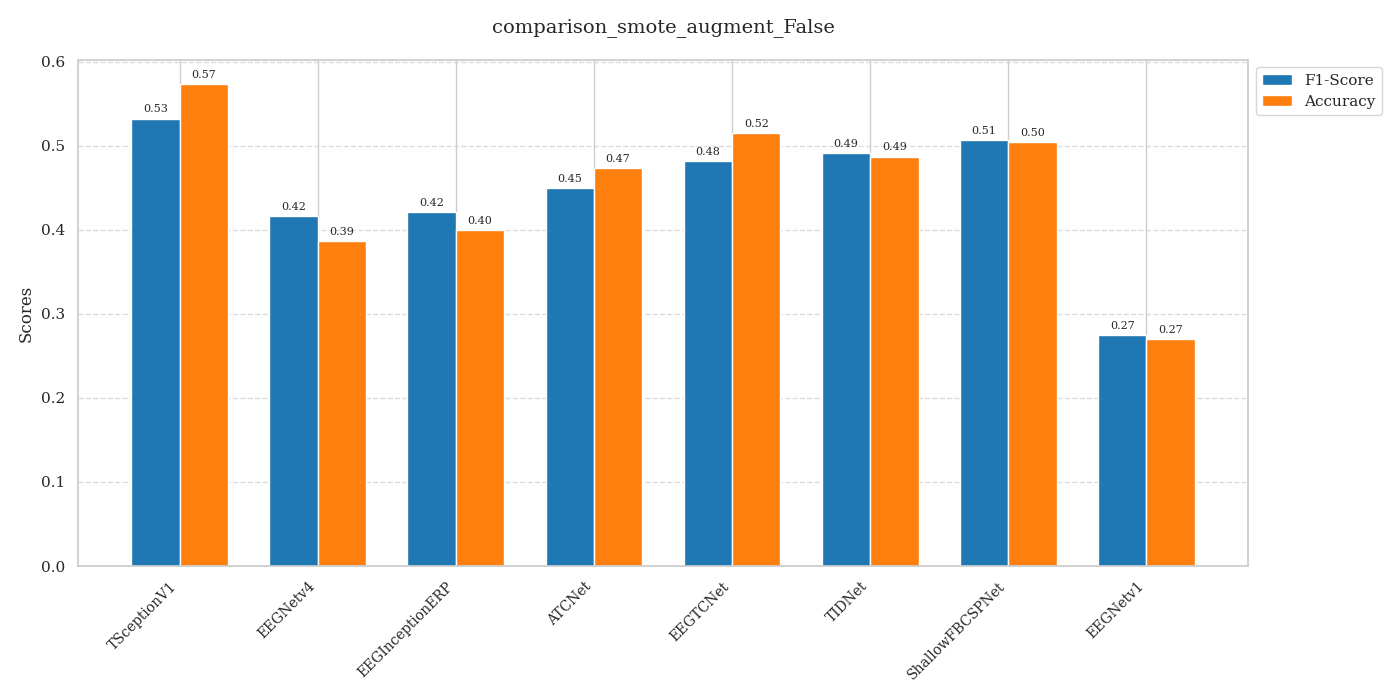
\includegraphics[width=1\linewidth]{images/comparison_smote_augment_False.png}
    \caption{Performanța modelelor folosind date sintetice, fără augmentări.}
    \label{fig:smote_augment_false}
\end{figure}

\begin{figure}
    \centering
    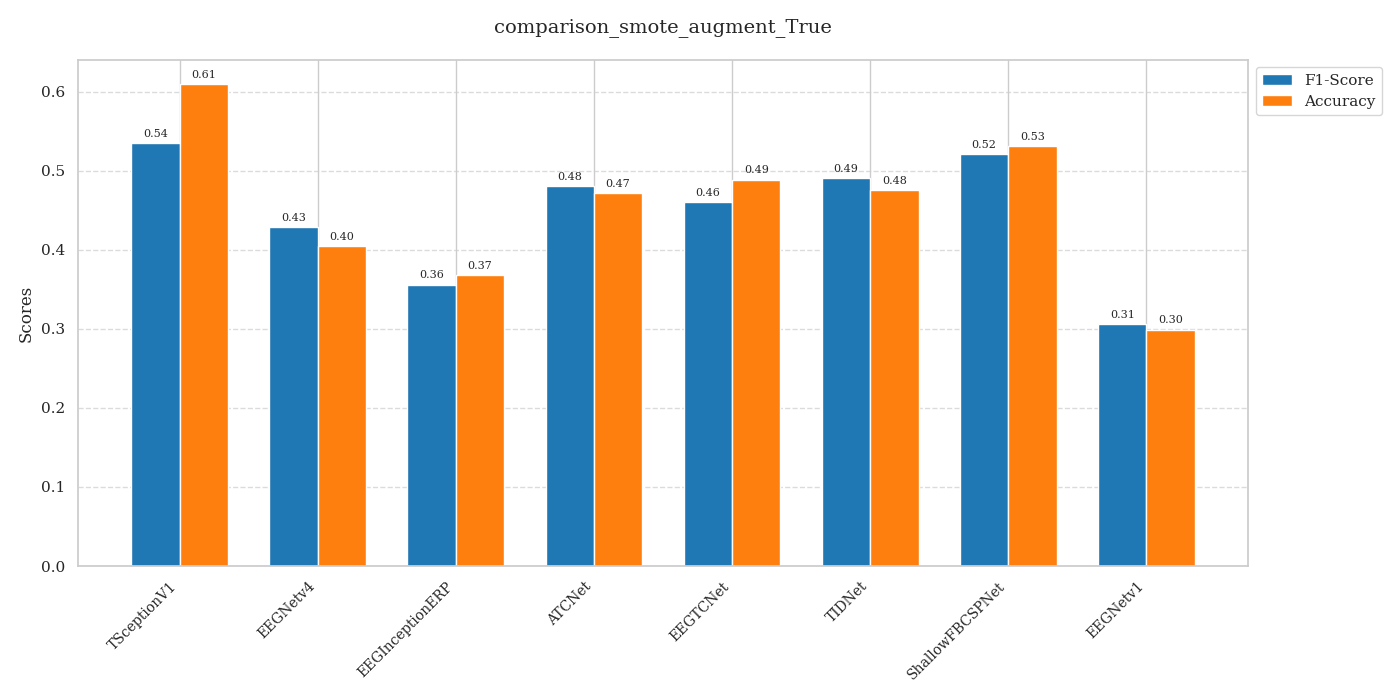
\includegraphics[width=1\linewidth]{comparison_smote_augment_True.png}
    \caption{Performanța modelelor, folosind date sintetice și augmentări.}
    \label{fig:smote_augment_true}
\end{figure}

\chapter{Cod sursă}

\begin{figure}[H]
\begin{lstlisting}[language=Python]
classifier = braindecode.classifier.EEGClassifier(
    model,
    criterion=torch.nn.CrossEntropyLoss,
    criterion__weight=torch.tensor(class_weights, dtype=torch.float32) if imbalance_mode=='class_weights' else None,
    train_split=predefined_split(torch.utils.data.TensorDataset(torch.tensor(X_valid).float(), torch.tensor(y_valid).long())),
    device='cuda',
    max_epochs=1000,
    callbacks=[skorch.callbacks.EarlyStopping(patience=20, load_best=True), skorch.callbacks.Checkpoint(), skorch.callbacks.LRScheduler()],
)
\end{lstlisting}
\caption{Apelarea wrapper-ului din braindecode.}
\label{fig:wrapper_braindecode}
\end{figure}

\begin{figure}[H]
\begin{lstlisting}[language=Python]
@ray.remote
def create_worker(participant, options):
    return EEGSubjectPipeline(participant, participant.replace("raw.csv", "quizz.xlsx"), 'dsi-24.elc', options)

workers = []
for participant in participants:
    workers.append(create_worker.remote(participant, options))

all_pipelines = ray.get(workers)

ray.shutdown()
\end{lstlisting}
\caption{Paralelizare utilizând Ray.}
\label{fig:paralelizare_ray}
\end{figure}


%\begin{figure}[h]
%    \centering
%    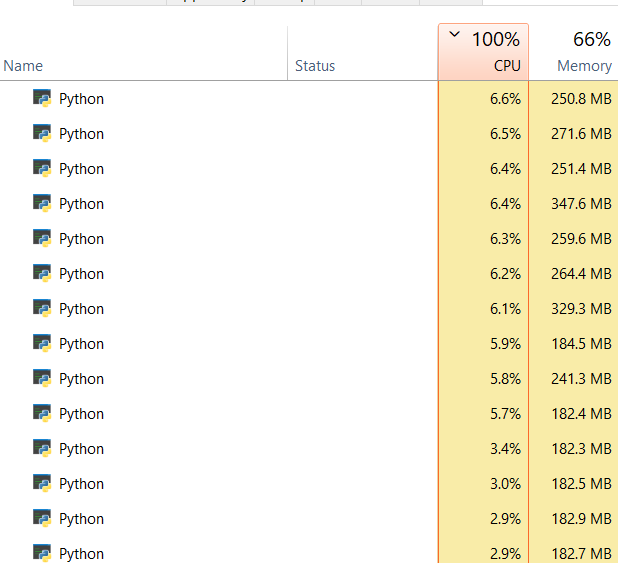
\includegraphics[width=0.7\linewidth]{task_manager.png}
%    \caption{Load-ul pe calculator}
%    \label{fig:load_calculator}
%\end{figure}

\begin{figure}
    \centering
    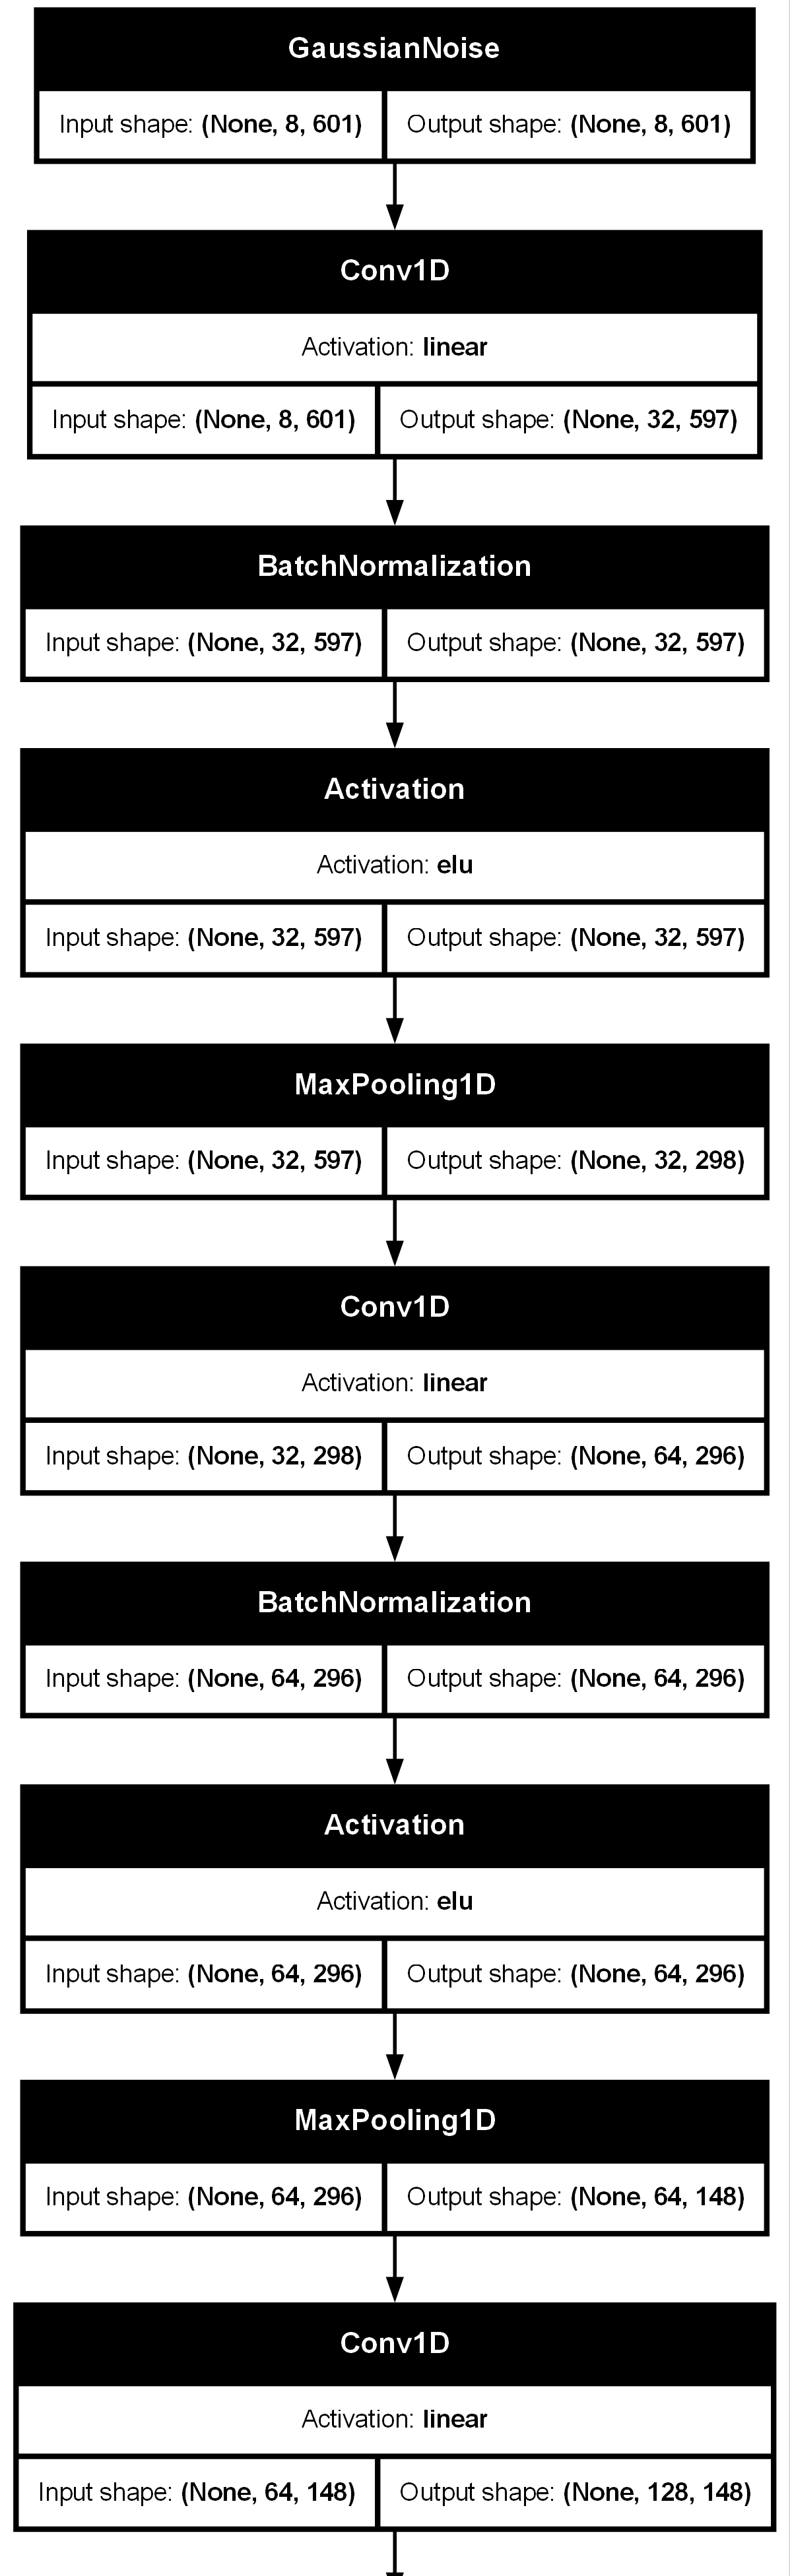
\includegraphics[width=0.4\linewidth]{model_part1.png}
    \caption{Model personal, partea 1.}
    \label{fig:model_part1}
\end{figure}

\begin{figure}
    \centering
    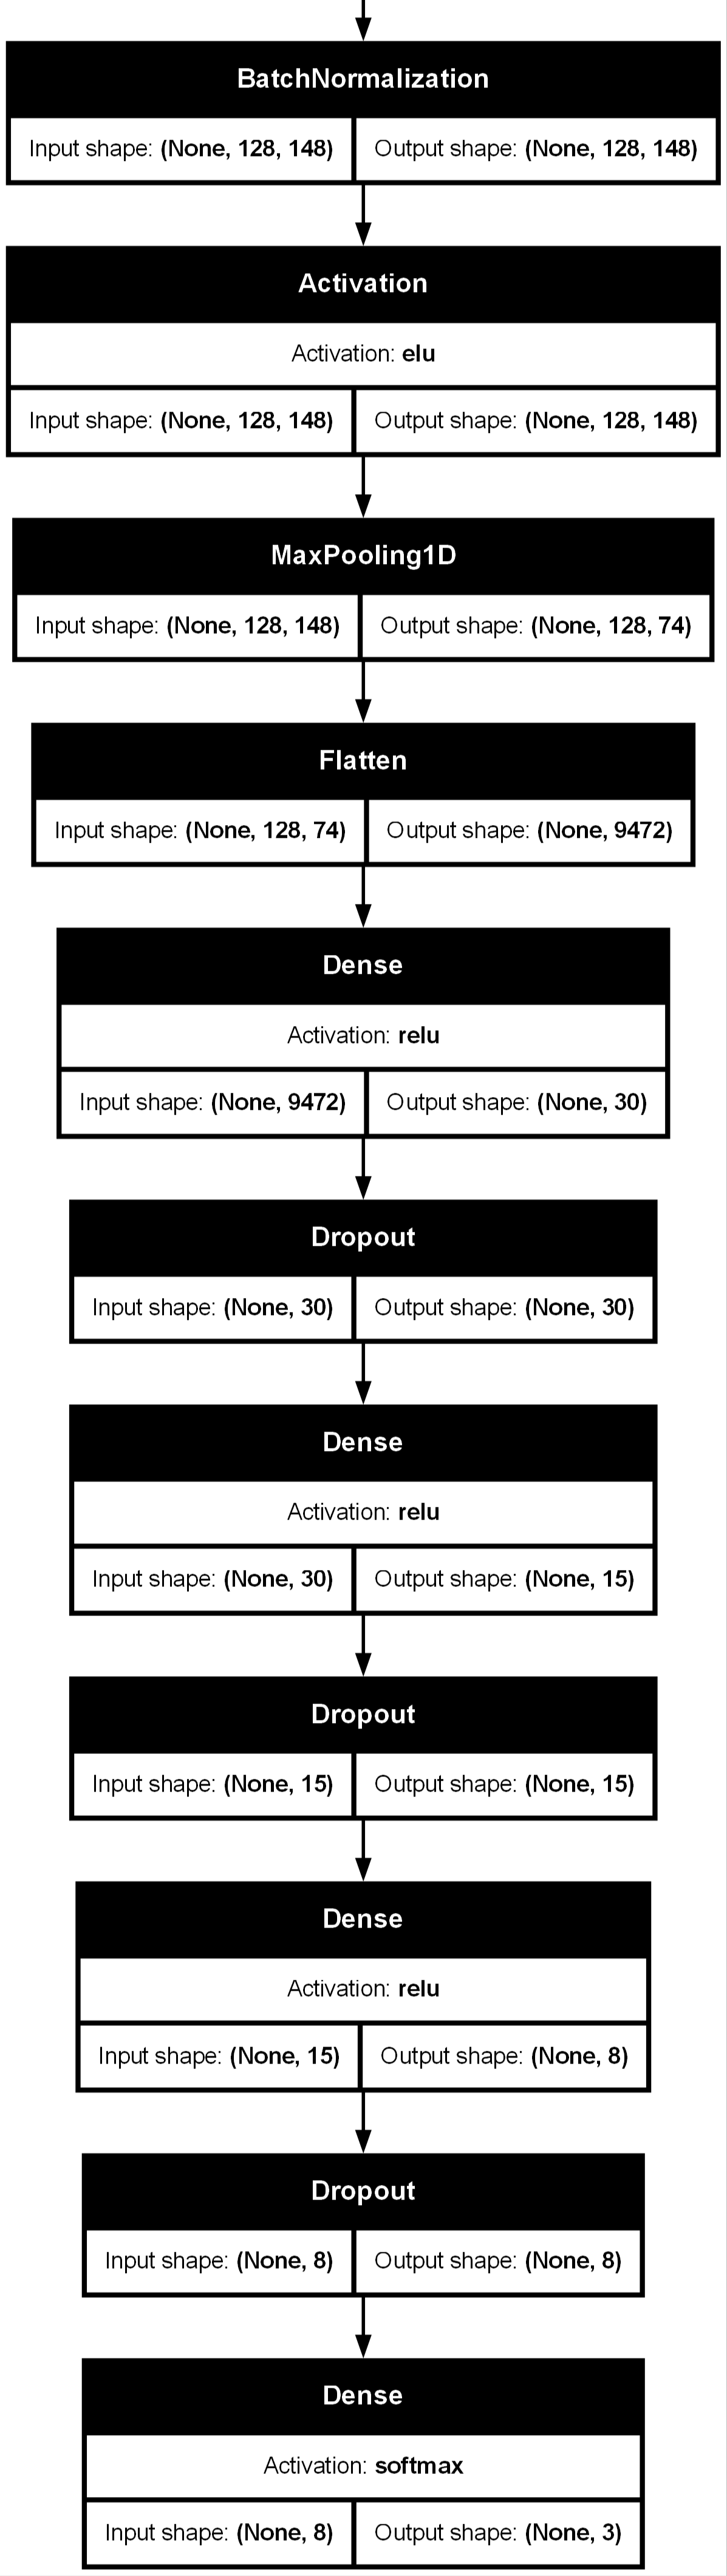
\includegraphics[width=0.4\linewidth]{model_part2.png}
    \caption{Model personal, partea 2.}
    \label{fig:model_part2}
\end{figure}

\begin{figure}
\begin{lstlisting}[language=Python]
def objective(trial):
    options = EEGpipelineOptions()

    options.interpolate_bad = trial.suggest_categorical('interpolate_bad', [False, True])
    options.apply_minmax_scaling_raw = trial.suggest_categorical('apply_minmax_scaling_raw', [False, True])
    options.apply_eog_regression = trial.suggest_categorical('apply_eog_regression', [False, True])
    options.apply_normalisation_raw = trial.suggest_categorical('apply_normalisation_raw', [False, True])
    options.apply_eeg_reference = trial.suggest_categorical('apply_eeg_reference', [False, True])

    options.apply_filters_raw = trial.suggest_categorical('apply_filters_raw', [False, True])
    options.apply_auto_ica_raw = False

    options.apply_manual_ica = False
    options.ica_components_raw = 20
    options.ica_threshold_raw = 2.5
    options.apply_autoreject = trial.suggest_categorical('apply_autoreject', [False, True])
    options.l_freq_raw = 4
    options.h_freq_raw = 40
    options.t_min = -0.2
    options.t_max = 1.8
    options.apply_xdawn_denoising = False
    options.apply_epoch_baseline = True

@ray.remote
def create_worker(participant, options):
    return EEGsubjectPipeline(participant, participant.replace("raw.csv", "quizz.xlsx"), "dsi-24.elc", options)

workers = []
for participant in participants:
    workers.append(create_worker_remote(participant, options))
all_pipelines = ray.get(workers)

ray.shutdown()

return get_model_metrics(braindecode.models.EEGNetv4(n_channels=n_chans, n_outputs=3, sfreq=300, n_times=601), all_pipelines)[1]

def callback(study, trial):
    if study.best_trial == trial:
        filehandler = open("output/braindecode_models/best_study.obj", "wb")
        pkl.dump(study, filehandler)
        filehandler.close()

study = optuna.create_study(direction="maximize")
study.optimize(objective, n_trials = 64, callbacks=[callback])
\end{lstlisting}
\caption{Cautarea hiperparametrilor folosind optuna.}
\label{fig:optuna_search}
\end{figure}

\begin{figure}
\begin{lstlisting}[language=Python]
def preprocess(self, apply_normalization = True, apply_minmax_scaling=True,
               apply_filters = True, apply_ica = True, apply_eog_regression = True,
               apply_manual_ica=True, apply_eeg_reference = True):
    if self.__isPreprocessed == True:
        return self
    self.__isPreprocessed = True
    if apply_eeg_reference:
        self.__apply_eeg_reference()
    if apply_filters:
        self.__filter_raw()
    if apply_eog_regression:
        self.__eog_regression()
    if apply_ica:
        self.__apply_auto_ica()
    if apply_manual_ica:
        self.__apply_ica()
    if apply_normalization:
        self.__normalize_raw()
    if apply_minmax_scaling:
        self.__minmax_scaling_raw()
    return self
\end{lstlisting}
\caption{Parametrizarea preprocesării semnalului.}
\label{fig:parametrizare}
\end{figure}

\begin{figure}
\begin{lstlisting}[language=Python]
if augment:
    X_train_jittered = add_temporal_jitter(X_train, jitter_range_ms=20, sampling_rate=300)
    X_train = np.concatenate([X_train, X_train_jittered], axis=0)
    y_train = np.concatenate([y_train, y_train], axis=0)

    X_train = torch.Tensor(X_train)
    y_train = torch.Tensor(y_train)
    X_train_noised, y_noised = braindecode.augmentation.GaussianNoise(probability=0.5) \
        .operation(X_train, y_train, std=0.1)
    X_train = X_train.detach().cpu().numpy()
    y_train = y_train.detach().cpu().numpy()

    X_train_noised = X_train_noised.detach().cpu().numpy()
    y_noised = y_noised.detach().cpu().numpy()
    X_train = np.concatenate([X_train, X_train_noised], axis=0)
    y_train = np.concatenate([y_train, y_noised], axis=0)

    X_train = torch.Tensor(X_train)
    y_train = torch.Tensor(y_train)
    X_train_noised, y_noised = braindecode.augmentation.SmoothTimeMask(probability=0.5) \
        .operation(X_train, y_train, mask_start_per_sample=torch.randint(low=0, high=400, size=(X_train.shape[0],)), 
                   mask_len_samples=40)
    X_train = X_train.detach().cpu().numpy()
    y_train = y_train.detach().cpu().numpy()

    X_train_noised = X_train_noised.detach().cpu().numpy()
    y_noised = y_noised.detach().cpu().numpy()
    X_train = np.concatenate([X_train, X_train_noised], axis=0)
    y_train = np.concatenate([y_train, y_noised], axis=0)
\end{lstlisting}
\caption{Codul folosit pentru agumentarea datelor.}
\label{fig:augmentari}
\end{figure}

\begin{figure}
\begin{lstlisting}[language=Python]
import pygad

all_features = ["mean", "variance", "std", "ptp_amp", "skewness", "kurtosis", "rms", "quantile", "hurst_exp",
                "app_entropy", "samp_entropy", "decorr_time", "pow_freq_bands", "hjorth_mobility_spect", "hjorth_complexity_spect",
                "hjorth_mobility", "hjorth_complexity", "higuchi_fd", "katz_fd", "zero_crossings", "line_length", "spect_slope",
                "spect_entropy", "svd_entropy", "svd_fisher_info", "energy_freq_bands", "spect_edge_freq", "wavelet_coef_energy",
                "teager_kaiser_energy"]

desired_output1 = 1
desired_output2 = 1

def fitness_func(ga_instance, solution, solution_idx):
    model = create_feature_pipeline(sklearn.neighbors.KNeighborsClassifier(), [x[0] for x in zip(all_features, solution) if x[1] > 0])
    output1, output2, _ = get_model_metrics(model, all_pipelines)
    return [output1, output2]

num_generations = 10
num_parents_mating = 10

sol_per_pop = 20
num_genes = len(all_features)

ga_instance = pygad.GA(num_generations=num_generations,
                       num_parents_mating = num_parents_mating,
                       sol_per_pop = sol_per_pop,
                       num_genes = num_genes,
                       fitness_func=fitness_func,
                       parent_selection_type='nsga2',
                       parallel_processing=('process', 8),
                       save_best_solutions=True,
                       save_solutions=True
                       )

ga_instance.run()
\end{lstlisting}
\caption{Configurația codului folosit pentru algoritmul genetic.}
\label{fig:pygad_configuration}
\end{figure}

\begin{figure}
\begin{lstlisting}[language=Python]
def create_pipeline(model):
    class Normalizer(sklearn.base.BaseEstimator, sklearn.base.TransformerMixin):
        def fit(self, X, y=None):
            self.mean = X.mean()
            self.std = X.std()
            return self

        def transform(self, X):
            return (X - self.mean) / self.std

    class FlattenTransformer(sklearn.base.BaseEstimator, sklearn.base.TransformerMixin):
        def fit(self, X, y=None):
            return self

        def transform(self, X):
            return X.reshape(X.shape[0], -1)

    steps = [("flatten", FlattenTransformer()), ("normalize", Normalizer()), ("scaler", sklearn.preprocessing.StandardScaler()), ("model", model)]
    pipe = Pipeline(steps)
    return pipe
\end{lstlisting}
\caption{Pipeline folosit pentru a normaliza și aplatiza datele trimise modelelor clasice.}
\label{fig:pipeline_modele_clasice}
\end{figure}